% Metódy inžinierskej práce

\documentclass[10pt,twoside,slovak,a4paper]{article}

\usepackage[slovak]{babel}
%\usepackage[T1]{fontenc}
\usepackage[IL2]{fontenc} % lepšia sadzba písmena Ľ než v T1
\usepackage[utf8]{inputenc}
\usepackage{graphicx}
\usepackage{url} % príkaz \url na formátovanie URL
\usepackage{hyperref} % odkazy v texte budú aktívne (pri niektorých triedach dokumentov spôsobuje posun textu)

\usepackage{cite}
%\usepackage{times}

\pagestyle{headings}

\title{Prečo e-šport existuje a prečo je taký drahý\thanks{Semestrálny projekt v predmete Metódy inžinierskej práce, ak. rok 2022/23, vedenie: Pavlo Balan}} % meno a priezvisko vyučujúceho na cvičeniach

\author{Balan Pavlo\\[2pt]
	{\small Slovenská technická univerzita v Bratislave}\\
	{\small Fakulta informatiky a informačných technológií}\\
	{\small \texttt{xbalan@stuba.sk}}
	}

\date{\small 05. october 2022} % upravte



\begin{document}

\maketitle

\begin{abstract}
\ldots
\end{abstract}



\section{Prečo ta tema?}

Minulý rok to bol najväčší esports turnaj DOTA 2 s prizepoolom 40 miliónov dolárov, kým predvlani sa na tom istom turnaji hralo takmer o 38 miliónov dolárov. Zaujímalo by ma, odkiaľ tieto peniaze pochádzajú a prečo sa esports rozvíja takým rýchlym tempom.

\begin{figure}[h]
	\centering
	\scalebox{0.4}{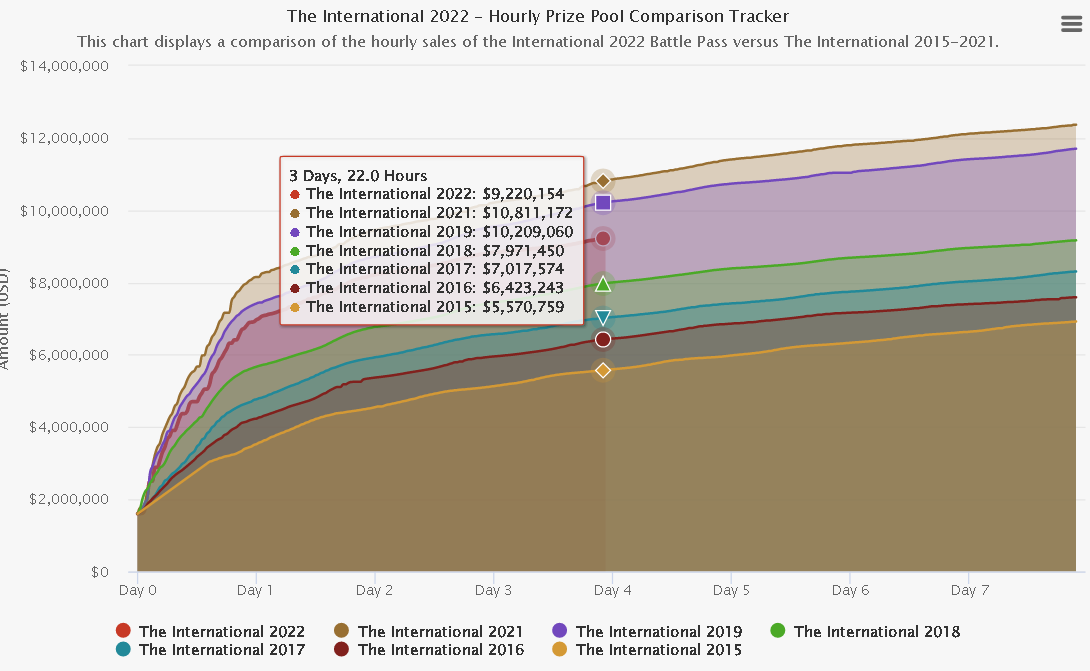
\includegraphics{prize.png}}
	\caption{Graf rastu prizepoolov na turnaji The international}
	\label{framework}
\end{figure}

\section{Pozadie} \label{nejaka}

Táto kapitola slúži ako úvod do sveta videohier pre viacerých hráčov, súťažné hry a e-športy.

\subsection{Hry pre viacerých hráčov}
Hra pre viacerých hráčov je, ako už názov napovedá, hra určená na hranie viacerých ľudí súčasne. Stolné hry a iné nedigitálne formy hry určené pre viacerých ľudí vyžadujú viac ako jedného aktívneho účastníka aby boli hrateľné. Napríklad šach sa má hrať a musí sa hrať súčasne dvomi osobami. Videohry na druhej strane už dávno majú schopnosť ponúknuť sa ako nevyhnutný protivník alebo protipól – často v nejakej forme umelej inteligencie alebo vopred navrhnutej hernej štruktúry. Prehrávanie a hra Tic-tac-toe na počítači, častejšie dáva príležitosť postaviť sa súperovi ovládanému AI namiesto toho, aby ste si museli nájsť kamaráta na hru s Koncept videohier pre viacerých hráčov teda nie je úplne samozrejmý ako si najskôr môžeme myslieť. Prvé multiplayerové videohry sa datujú už do roku 1958, kedy boli americké fyzik William Higinbotham vyvinul tenisový simulátor Tennis for Two navrhnutý pre analógový počítač Donner Model 30. Hra obsahovala dva ručné ovládače a päťpalcový osciloskopový monitor na hranie. Je široko považovaná za jednu z úplne prvých elektronických hier zobrazujúcich pohyb [9] a je následne jedna z úplne prvých hier pre viacerých hráčov, odkedy bola navrhnutá hrané medzi dvoma ľuďmi. V roku 1972 klasická hra Atari Pong urobila hry pre viacerých hráčov ešte viac populárny. Pong položil základy toho, čo sa nazýva zlatý vek arkádových videohier, pretože to bola jedna z prvých hier, ktoré sa hrali v arkádových hrách skrine a súčasne prvá úspešná komerčná videohra vôbec [8]. Tenis pre dvoch aj Pong vychádzali z tenisu, aj keď mali rôzne grafické prístupy – prvý stvárnil tenisový kurt z r strane a to druhé zhora. Hry pre viacerých hráčov a športy v reálnom živote zdieľajú a veľa základných vlastností, takže nie je prekvapujúce, že medzi ne patrili aj športové hry prvé videohry pre viacerých hráčov, ktoré navrhli vývojári hier. V nasledujúcich rokoch sa vyvinula široká škála typov hier pre viacerých hráčov. Strieľačky z pohľadu prvej osoby boli vždy populárne, rovnako ako strategické hry v reálnom čase. Niektoré hry, ktoré sú primárne vytvorené ako hry pre jedného hráča, sa niekedy dodávajú a režim hry pre viacerých hráčov, aby rozšírili svoj podiel na trhu. Môže tiež predĺžiť životnosť hry, ako je to pri Diablo II (Blizzard Entertainment, 2000). ~\cite{Bornemark:SFfEG}
\subsection{Competitive Gaming and E-sport} 
As multiplay video games became more and more popular, people started to compete against each other in a more serious way. The spread of personal computers made more people able to play and the rapid development of the Internet and game net-code allowed for lower in-game latency between gamers. E-sport Success Factors for E-Sport Games 3 mainly focuses on competition and although in general any computer game that allows playing against another could be a possible discipline in e-sport, there are certain core games, which are most popular even from a worldwide perspective. The classic game Doom (id Software, 1993) laid the foundation of competitive gaming for the PC and its sequel Doom II (1994) was the game of choice for one of the first offline PC gaming tournaments ever: Deathmatch ’95 in 1995. Ever since, tournaments of all sizes have emerged. Some are trying to claim the title as the “world championships”, such as The World Cyber Games, Electronic Sports World Cup and World eSports Games, similar to how there are many “world titles” in professional boxing. The term “e-sports” or “electronic sports” dates back to the late nineties. In Asia, and particularly South Korea, e-sports culture have taken a firm grip of society. Since its release in 1998, the game StarCraft (Blizzard Entertainment) has since been the center pillar of gaming in the country, allowing for highly paid professional players and dedicated national television channels, broadcasting the game. Today, e-sport is either recognized or accepted as a sport in over 60 countries around the world, especially in Asian countries.

\section{Iná časť} \label{ina}

Základným problémom je teda\ldots{} Najprv sa pozrieme na nejaké vysvetlenie (časť~\ref{ina:nejake}), a potom na ešte nejaké (časť~\ref{ina:nejake}).\footnote{Niekedy môžete potrebovať aj poznámku pod čiarou.}

Môže sa zdať, že problém vlastne nejestvuje\cite{Coplien:MPD}, ale bolo dokázané, že to tak nie je~\cite{Czarnecki:Staged, Czarnecki:Progress}. Napriek tomu, aj dnes na webe narazíme na všelijaké pochybné názory\cite{PLP-Framework}. Dôležité veci možno \emph{zdôrazniť kurzívou}.


\subsection{Nejaké vysvetlenie} \label{ina:nejake}

Niekedy treba uviesť zoznam:

\begin{itemize}
\item jedna vec
\item druhá vec
	\begin{itemize}
	\item x
	\item y
	\end{itemize}
\end{itemize}

Ten istý zoznam, len číslovaný:

\begin{enumerate}
\item jedna vec
\item druhá vec
	\begin{enumerate}
	\item x
	\item y
	\end{enumerate}
\end{enumerate}


\subsection{Ešte nejaké vysvetlenie} \label{ina:este}

\paragraph{Veľmi dôležitá poznámka.}
Niekedy je potrebné nadpisom označiť odsek. Text pokračuje hneď za nadpisom.



\section{Dôležitá časť} \label{dolezita}




\section{Ešte dôležitejšia časť} \label{dolezitejsia}




\section{Záver} \label{zaver} % prípadne iný variant názvu



%\acknowledgement{Ak niekomu chcete poďakovať\ldots}


% týmto sa generuje zoznam literatúry z obsahu súboru literatura.bib podľa toho, na čo sa v článku odkazujete
\bibliography{literatura}
\bibliographystyle{plain} % prípadne alpha, abbrv alebo hociktorý iný
\end{document}
